Das erzeugte Streifenmuster in Abbildung \ref{img:differenceCamPat} hat nicht mehr den Grauwerteverlauf einer Rechteckschwingung (vgl. Abbildung \ref{tikz:abbRechteckschwingung}) entlang der Ausbreitungsrichtung.
Dadurch lässt sich das Streifenmuster nicht mehr in der Form aus Gleichung \ref{eq:rstreifenmuster} darstellen.
Der Grauwerteverlauf in einer Zeile bzw. Spalte eines solchen Streifenmusters entspricht einer Impulsschwingung (siehe Abbildung \ref{tikz:abbPulsewave}).
%
% Abbildung: Pulswave
{
	\begin{figure}[H]
		\centering
		\begin{adjustbox}{width=\textwidth}
	\begin{tikzpicture}
	
		% Koordinatensystem
		\draw[thick,-stealth,black] (0,0)--(16,0) node[below] {$x$};
		\draw[thick,-stealth,black] (0,0)--(0,4.25) node[left] {$m_1(x,y_0)$};
		\draw[thick,black] (0,0) -- (0,-0.1) node[anchor=north,fill=white] {$0$};
		\draw[thick,black] (15,0) -- (15,-0.1) node[anchor=north,fill=white] {\acrshort{lwidth}};
		\draw[thick,black] (0,0) -- (-0.1,0) node[anchor=east,fill=white] {$0$};
		\draw[thick,black] (0,3.75) -- (-0.1,3.75) node[anchor=east,fill=white] {$255$};

		% Funktion, erste Periode
		\draw[blue, thick] (0,3.75) -- (1,3.75);
		\draw[blue, thick] (1,3.75) -- (1,0);
		\draw[blue, thick] (1,0) -- (3.75,0);
		\draw[blue, thick] (3.75,0) -- (3.75,3.75);
		
		% Funktion, zweite Periode
		\draw[blue, thick] (3.75,3.75) -- (4.75,3.75);
		\draw[blue, thick] (4.75,3.75) -- (4.75,0);
		\draw[blue, thick] (4.75,0) -- (7.5,0);
		\draw[blue, thick] (7.5,0) -- (7.5,3.75);
		
		% Funktion, dritte Periode
		\draw[blue, thick] (7.5,3.75) -- (8.5,3.75);
		\draw[blue, thick] (8.5,3.75) -- (8.5,0);
		\draw[blue, thick] (8.5,0) -- (11.25,0);
		\draw[blue, thick] (11.25,0) -- (11.25,3.75);
		
		% Funktion, vierte Periode
		\draw[blue, thick] (11.25,3.75) -- (12.25,3.75);
		\draw[blue, thick] (12.25,3.75) -- (12.25,0);
		\draw[blue, thick] (12.25,0) -- (15,0);

		\end{tikzpicture}
\end{adjustbox}
\caption[Impulsschwingung bzw. \textit{eng: pulse wave, rectangular wave}]{Impulsschwingung, \textit{eng: pulse wave, rectangular wave}, eines Streifenmusters mit Ausbreitungsrichtung in $x$ bei fester, aber beliebiger Zeile $y_0$.}
		\label{tikz:abbPulsewave}
	\end{figure}
}
%
\noindent
Um eine Gleichung für eine solche Impulsschwingung (siehe Abbildung \ref{tikz:abbPulsewave}) herzuleiten, kann man die periodische Sägezahnschwingung verwenden \cite{waveGeneration}.
Eine Sägezahnschwingung lässt sich darstellen durch (vgl. \cite{sawtoothWave}):
%
\begin{equation} \label{eq:saegezahnschwingung}
	w_f(t) = 2 \left( ft - \left\lfloor ft \right\rfloor \right) - 1
\end{equation}
%
\noindent
$f$ bezeichnet die Frequenz der Sägezahnschwingung und steht analog zu Gleichung \ref{eq:einheitsrechteckschwingung} über den Kehrwert im Zusammenhang mit der Periodenlänge der Sägezahnschwingung $w_f(t)$:
%
\begin{equation*}
	f = \dfrac{1}{T}
\end{equation*}
%
Mit $T = 3$ erhält man folgendes Schaubild (siehe Abbildung \ref{tikz:abbsaegezahnSchwingung}).
%
% Abbildung: Sägezahnschwingung
{
	\begin{figure}[H]
		\centering
		\input{03_sichtpruefungDurchLichtstreuung/optimierungen/musterMitUnterschiedlichenStreifenbreiten/figures/abbSaegezahnSchwingung}
		\label{tikz:abbsaegezahnSchwingung}
	\end{figure}
}
%
\noindent
Bildet man die Differenz von zwei zueinander versetzten Sägezahnfunktionen, erhält man die Impulsschwingung $p_{f,D}(t)$:
%
\begin{equation} \label{eq:pulsewave}
	p_{f,D}(t) = w_f(t - \dfrac{D}{f}) - w_f(t) - w_f(- \dfrac{D}{f}),
	\quad
	D \in \left(0,1\right] \subset \acrshortmath{real}
\end{equation}
%
\noindent
$D$ wird Tastgrad (\textit{engl: duty cycle}) genannt und bezeichnet die Impulsdauer der Impulsschwingung im Verhältnis zur Periodenlänge $T$.
Somit erhält man mit $D = \tfrac{1}{2}$ eine Rechteckschwingung wie auch in Abbildung \ref{tikz:abbRechteckschwingung}.
Ein Schaubild der Gleichung \ref{eq:pulsewave} wird in Abbildung \ref{tikz:abbNormalPulsewave} dargestellt.
%
% Abbildung: Normale Impulsschwingung
{
	\begin{figure}[H]
		\centering
		\begin{adjustbox}{width=\textwidth}
	\begin{tikzpicture}[declare function={sawtooth(\x) = 1.5*(2*((\x/3)-0.5-floor((\x/3))));}]
	
		% Koordinatensystem
		\draw[thick,-stealth,black] (-8,0)--(8,0) node[below] {$t$};
		\draw[thick,-stealth,black] (0,-2.125)--(0,2.125) node[left] {$p_{\tfrac{1}{3},\tfrac{1}{3}}(t)$};
		
		% Funktion
		\draw[name path = func1, blue, thick, domain=-8:8, samples=600] plot (\x, {sawtooth(\x - (1/3) * 3) - sawtooth(\x) - sawtooth(-(1/3) * 3)});
		
		% Achsenbeschriftungen
		\draw[thick,black] (0,-1.5) -- (-0.1,-1.5) node[anchor=east,fill=white] {$-1$};
		\draw[thick,black] (0,1.5) -- (-0.1,1.5) node[anchor=east,fill=white] {$1$};
		\draw[thick,black] (-7,0) -- (-7,-0.1) node[anchor=north,fill=white] {$-7$};
		\draw[thick,black] (-6,0) -- (-6,-0.1) node[anchor=north,fill=white] {$-6$};
		\draw[thick,black] (-5,0) -- (-5,-0.1) node[anchor=north,fill=white] {$-5$};
		\draw[thick,black] (-4,0) -- (-4,-0.1) node[anchor=north,fill=white] {$-4$};
		\draw[thick,black] (-3,0) -- (-3,-0.1) node[anchor=north,fill=white] {$-3$};
		\draw[thick,black] (-2,0) -- (-2,-0.1) node[anchor=north,fill=white] {$-2$};
		\draw[thick,black] (-1,0) -- (-1,-0.1) node[anchor=north,fill=white] {$-1$};
		\draw[thick,black] (1,0) -- (1,-0.1) node[anchor=north,fill=white] {$1$};
		\draw[thick,black] (2,0) -- (2,-0.1) node[anchor=north,fill=white] {$2$};
		\draw[thick,black] (3,0) -- (3,-0.1) node[anchor=north,fill=white] {$3$};
		\draw[thick,black] (4,0) -- (4,-0.1) node[anchor=north,fill=white] {$4$};
		\draw[thick,black] (5,0) -- (5,-0.1) node[anchor=north,fill=white] {$5$};
		\draw[thick,black] (6,0) -- (6,-0.1) node[anchor=north,fill=white] {$6$};
		\draw[thick,black] (7,0) -- (7,-0.1) node[anchor=north,fill=white] {$7$};	
		
	\end{tikzpicture}
\end{adjustbox}
\caption[Einheits-Impulsschwingung]{Einheits-Impulsschwingung nach Gleichung \ref{eq:pulsewave} mit $f = \tfrac{1}{3}$ und $D = \tfrac{1}{3}$.}
		\label{tikz:abbNormalPulsewave}
	\end{figure}
}
%
\noindent
Aus Gleichung \ref{eq:pulsewave} lässt sich somit eine mathematische Darstellung für Streifenmuster mit unterschiedlichen Streifenbreiten aufschreiben:
%
\begin{equation} \label{eq:impulsStreifenmuster}
	\begin{gathered}
		m_k(x,y) = A_m \left( 1 + p_{f,D}\left( x - \dfrac{1}{2 \pi f} \psi_k \right) \right),
		\\
		f = \dfrac{N_p}{\acrshortmath{lwidth}},
		\quad
		D \in \left(0,1\right] \subset \acrshortmath{real},
		\quad
		\psi_k = (k - 1)\dfrac{2\pi}{N_{shift}},
		\quad
		k \in \lbrace 1,\ldots,N_{shift}\rbrace
	\end{gathered}
\end{equation}
%
Wie auch in Gleichung \ref{eq:rstreifenmuster} gilt für dieses Muster die Periodizität in der Ausbreitungsrichtung.
Auch hier bezeichnet $A_m$ die Amplitude, $N_p$ die Anzahl der Perioden über die Monitorbreite \acrshort{lwidth}, $N_{shift}$ die Anzahl der Phasenverschiebungen und $\psi_k$ die Phasenverschiebung des $k$-ten Musters.
Zusätzlich zu diesen Parametern hat man den Tastgrad $D$, der in diesem Fall die Breite der hellen Streifen im Verhältnis zu der Periodenlänge $T$ angibt.
Die Periodenlänge $T$ ist im Streifenmuster die Summe der Breite eines einzelnen dunklen und eines einzelnen hellen Streifens.
Analog zu Gleichung \ref{eq:impulsStreifenmuster} lässt sich auch ein horizontales Streifenmuster mit Ausbreitungsrichtung in $y$ über die Monitorhöhe \acrshort{lheight} aufschreiben.
Das Bild eines vertikalen Streifenmusters, d. h. mit Ausbreitungsrichtung in $x$, nach Gleichung \ref{eq:impulsStreifenmuster} wird in Abbildung \ref{img:impulsschwingungStreifenmuster} dargestellt.
%
\begin{figure}[H]
	\centering
	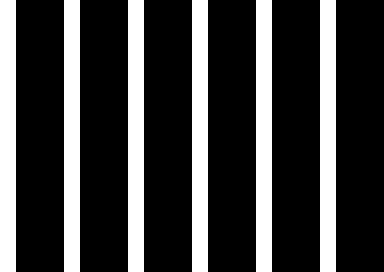
\includegraphics[frame,width=0.5\textwidth]{03_sichtpruefungDurchLichtstreuung/optimierungen/musterMitUnterschiedlichenStreifenbreiten/figures/impulsschwingungStreifenmuster}
	\caption[Rechteckförmiges Streifenmuster]{Streifenmuster nach Gleichung \ref{eq:rstreifenmuster}, mit $A_m = 127.5$, $N_p = 6$, $\acrshortmath{lwidth} = 384$, $D = \tfrac{1}{4}$ und $\psi_1 = 0$. Die hellen Streifen haben damit eine Breite von 16 Pixeln und die dunklen Streifen eine Breite von 48 Pixeln.}
	\label{img:impulsschwingungStreifenmuster}
\end{figure}